\documentclass[tikz]{standalone}
\usepackage{pgfplots}
\pgfplotsset{compat=1.15}
\usepackage{mathrsfs}
\usetikzlibrary{arrows,calc}
\usepackage{tkz-euclide}

\pagestyle{empty}

\definecolor{AngleClr}{rgb}{0,0.39215686274509803,0}
\definecolor{ShapeClr}{rgb}{0.6,0.2,0}
\definecolor{BlueClr}{RGB}{5,81,163}

\begin{document}

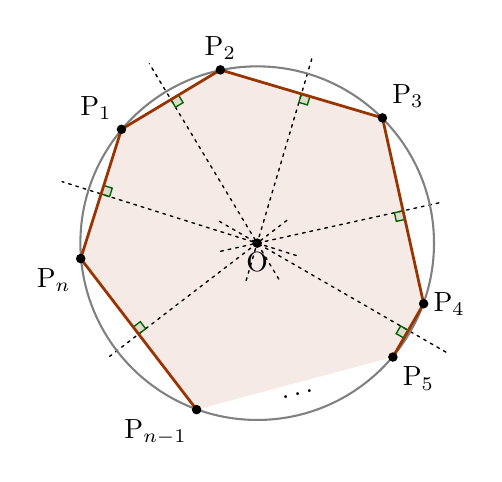
\begin{tikzpicture}[scale=.75]
\tkzSetUpLine[line width=1pt,color=black]
\tkzSetUpPoint[fill=black]

\tkzDefPoint(140:3){P1}
\tkzDefPoint(102:3){P2}
\tkzDefPoint(45:3){P3}
\tkzDefPoint(-20:3){P4}
\tkzDefPoint(-40:3){P5}
\tkzDefPoint(-110:3){Pnn}
\tkzDefPoint(-175:3){Pn}


\tkzDefTriangleCenter[circum](P1,P2,P3) \tkzGetPoint{O}

\tkzDefMidPoint(Pnn,Pn) \tkzGetPoint{M1}
\tkzDefMidPoint(Pn,P1) \tkzGetPoint{M2}
\tkzDefMidPoint(P1,P2) \tkzGetPoint{M3}
\tkzDefMidPoint(P2,P3) \tkzGetPoint{M4}
\tkzDefMidPoint(P3,P4) \tkzGetPoint{M5}
\tkzDefMidPoint(P4,P5) \tkzGetPoint{M6}

\tkzFillPolygon[fill=ShapeClr,fill opacity=0.1](P1,P2,P3,P4,P5,Pnn,Pn)
\tkzDrawSegments[line width=0.5pt,color=black,dashed,dash pattern=on 1pt off 1.75pt,add=0.25 and 0.25](O,M1 O,M2 O,M3 O,M4 O,M5 O,M6)

\tkzMarkRightAngles[line width=0.5pt, size=.15,color=AngleClr,fill=AngleClr,fill opacity=0.1](O,M1,Pn O,M2,P1 O,M3,P2 O,M4,P3 O,M5,P4 O,M6,P5)

\tkzDrawCircle[line width=0.75](O,P1)


\tkzDrawSegments[line width=1pt,color=ShapeClr](Pnn,Pn Pn,P1 P1,P2 P2,P3 P3,P4 P4,P5)

\tkzLabelSegment[sloped](Pnn,P5){$\ldots$}

\tkzDrawPoints[size=3](P1,P2,P3,P4,P5,Pnn,Pn,O)
\tkzLabelPoint[above left](P1){${\rm P}_1$}
\tkzLabelPoint[above](P2){${\rm P}_2$}
\tkzLabelPoint[above right](P3){${\rm P}_3$}
\tkzLabelPoint[right](P4){${\rm P}_4$}
\tkzLabelPoint[below right](P5){${\rm P}_5$}
\tkzLabelPoint[below left](Pnn){${\rm P}_{n-1}$}
\tkzLabelPoint[below left](Pn){${\rm P}_{n}$}
\tkzLabelPoint[below](O){$\rm O$}

\end{tikzpicture}

\end{document}
